\subsection{Key Results}
\label{section:main_results}

We compare \ours\ to the following SoTA multivariate baselines: (1) \FEDformer~\citep{zhouFEDformer2022}, (2) \Autoformer~\citep{wu2021autoformer}, (3) \Informer~\citep{zhou2021informer}, (4) \Reformer~\citep{kitaev2020reformer} and (5) \LogTrans~\citep{li2019logtrans}. Additionally, we consider the univariate baselines: (6) \DilRNN~\citep{chang2017dilatedRNN} and (7) auto-\ARIMA~\citep{hyndman2008automatic_arima}.

\begin{figure}[t] %!ht
    \centering
    \subfigure[\emph{Time Efficiency}]{\label{fig:inference_comparison}
    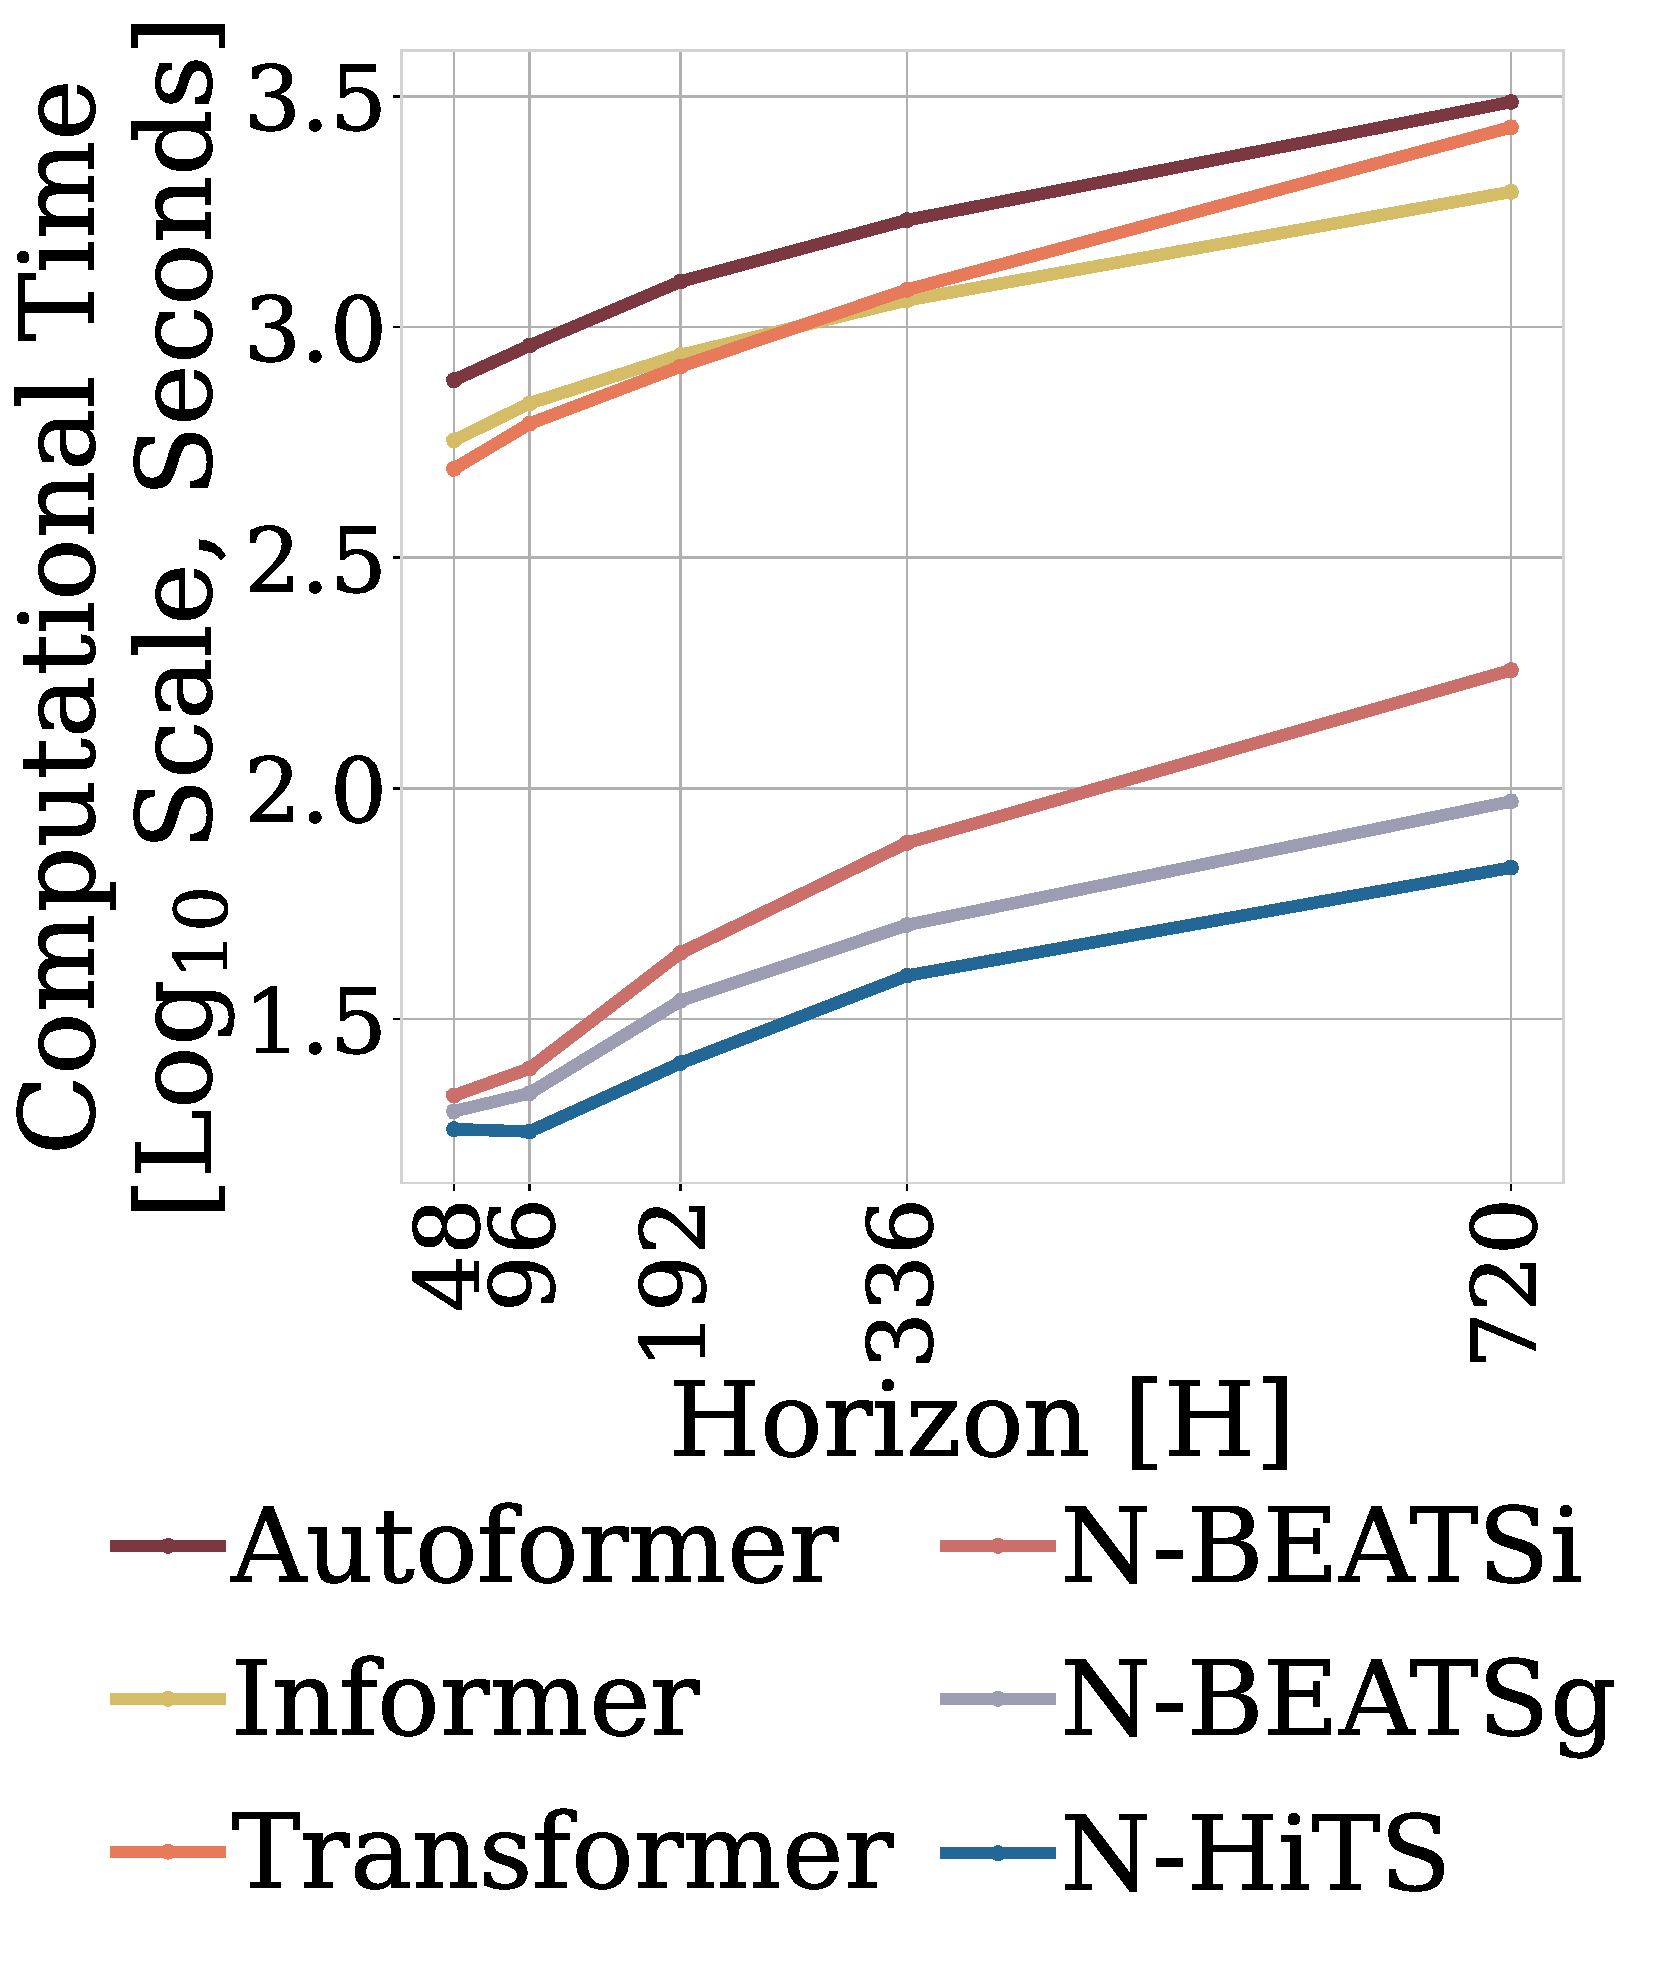
\includegraphics[width=0.4\linewidth]{images/plots-comparison-time.pdf}} %0.472
    \hspace{10mm} 
    \subfigure[\emph{Memory Efficiency}]{\label{fig:memory_comparison}
    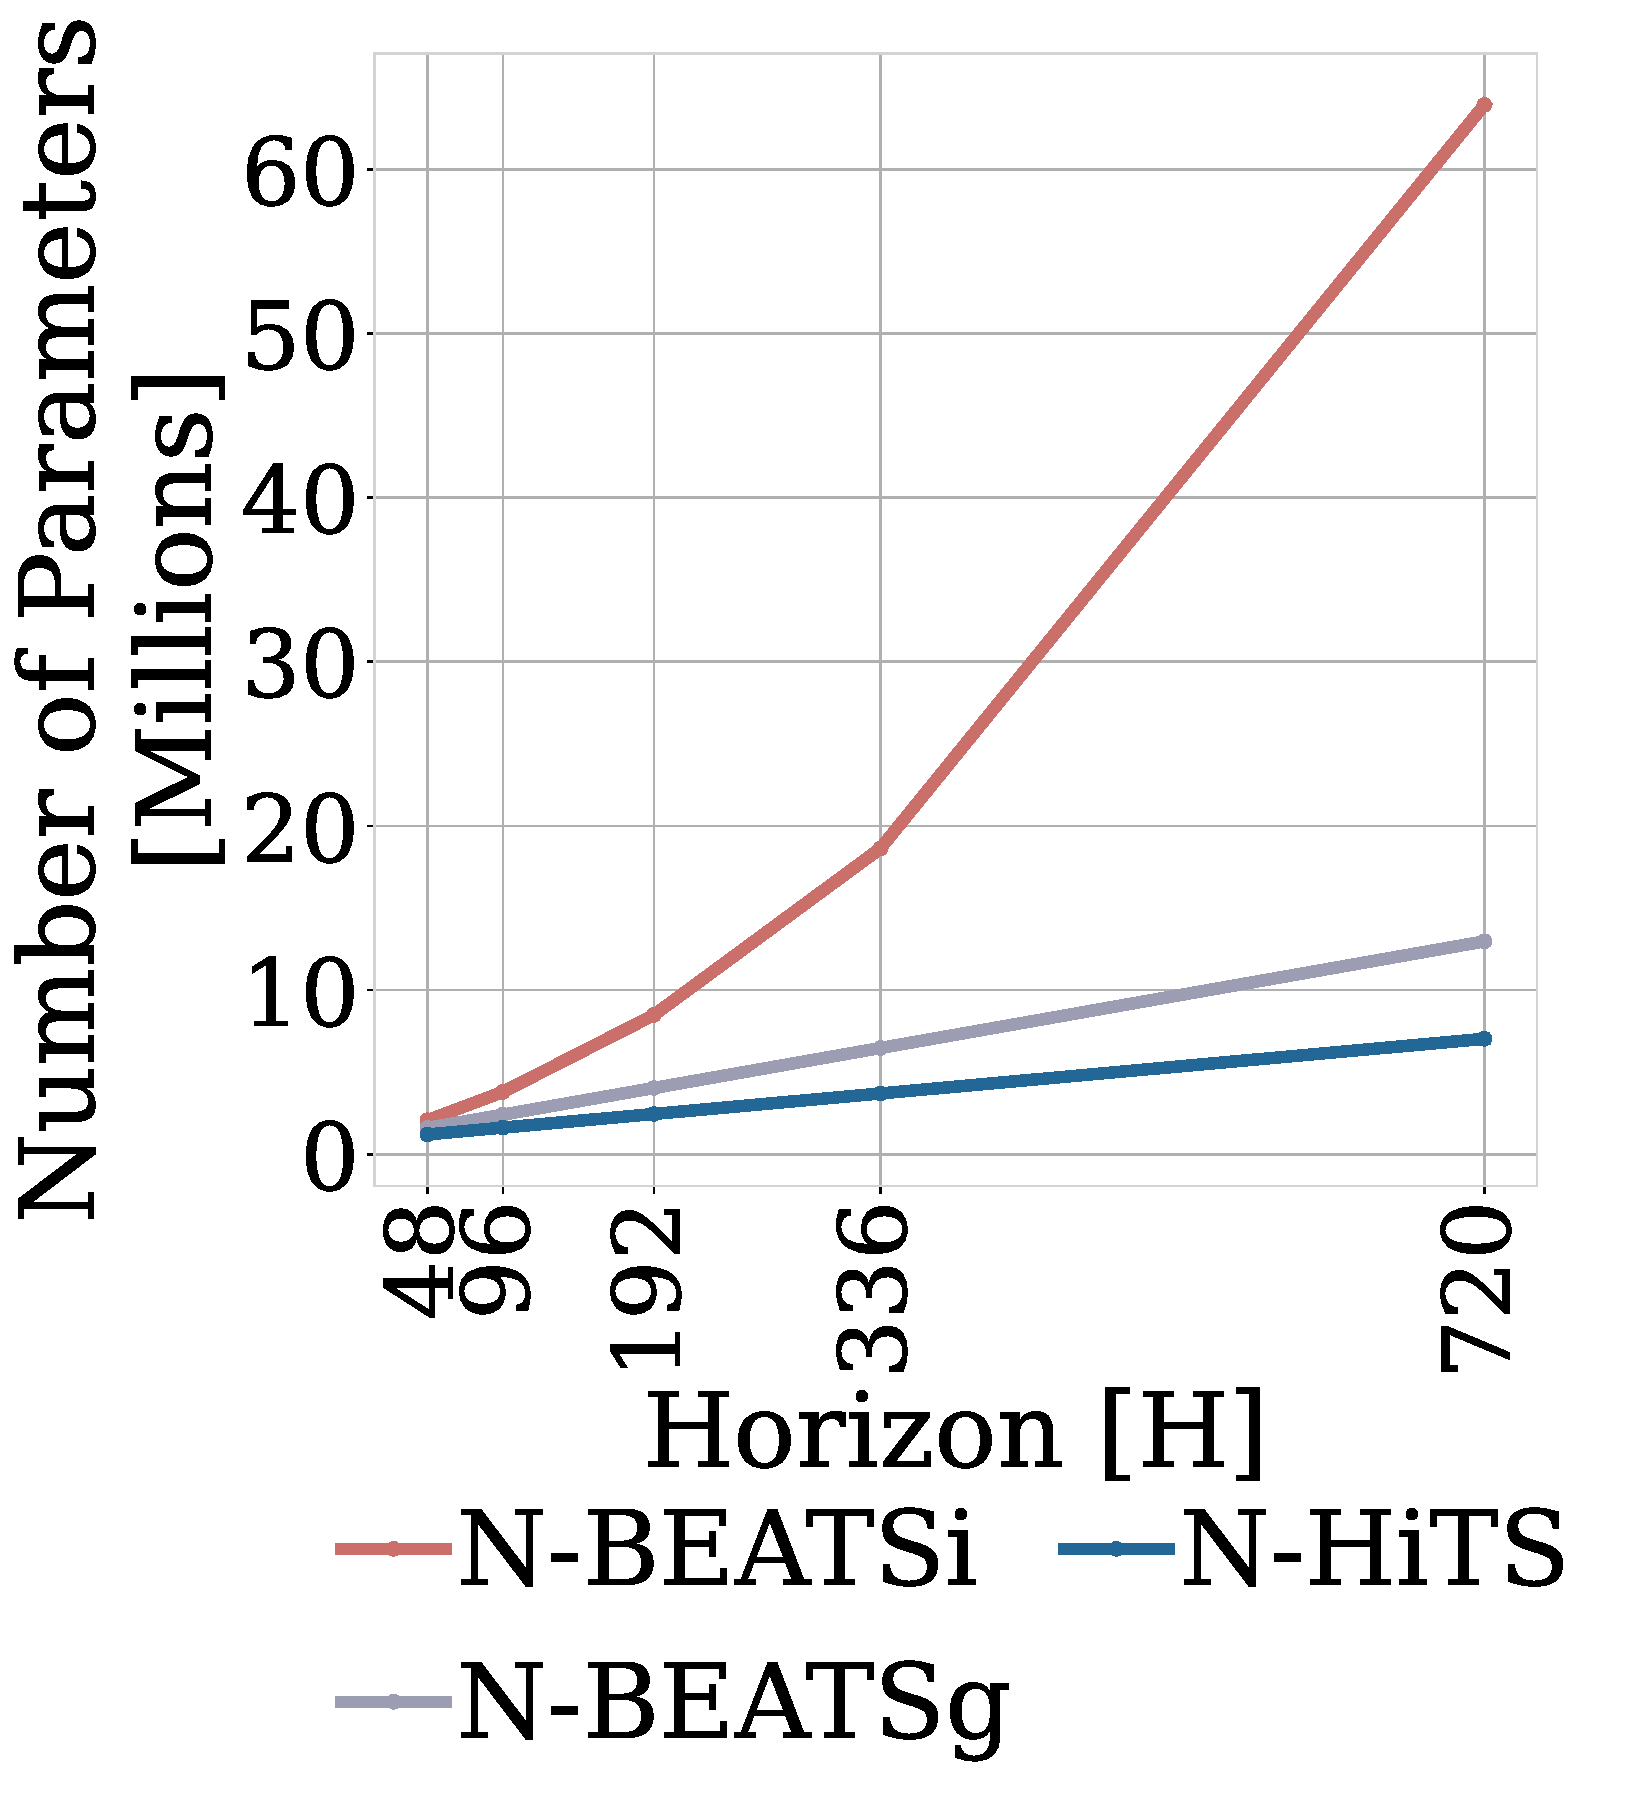
\includegraphics[width=0.4\linewidth]{images/plots-comparison-params.pdf}} % 0.495
    %\vspace{-0.5cm}
    \caption{Computational efficiency comparison. \ours\ exhibits the best training time compared to Transformer-based and fully connected models, and smallest memory footprint.}
    \label{fig:computational_cost_comparison}
\end{figure}

\textbf{Forecasting Accuracy.} Table~\ref{table:main_results_multivar} summarizes the multivariate forecasting results. \ours\ outperforms the best baseline, with average relative error decrease across datasets and horizons of \multivarMAEgains\% in MAE and \multivarMSEgains\% in MSE. \ours\ maintains a comparable performance to other state-of-the-art methods for the shortest measured horizon (96/24), while for the longest measured horizon (720/60) decreases multivariate MAE by \multivarlongMAEgains\% and MSE by \multivarlongMSEgains\%. We complement the key results in Table~\ref{table:main_results_multivar}, with the additional univariate forecasting experiments in Appendix F, again demonstrating state-of-the-art performance against baselines.

\begin{figure*}[ht!]
\centering
\subfigure[H. interpolation, multi-rate sampling]{\label{fig:decomposition_mf}
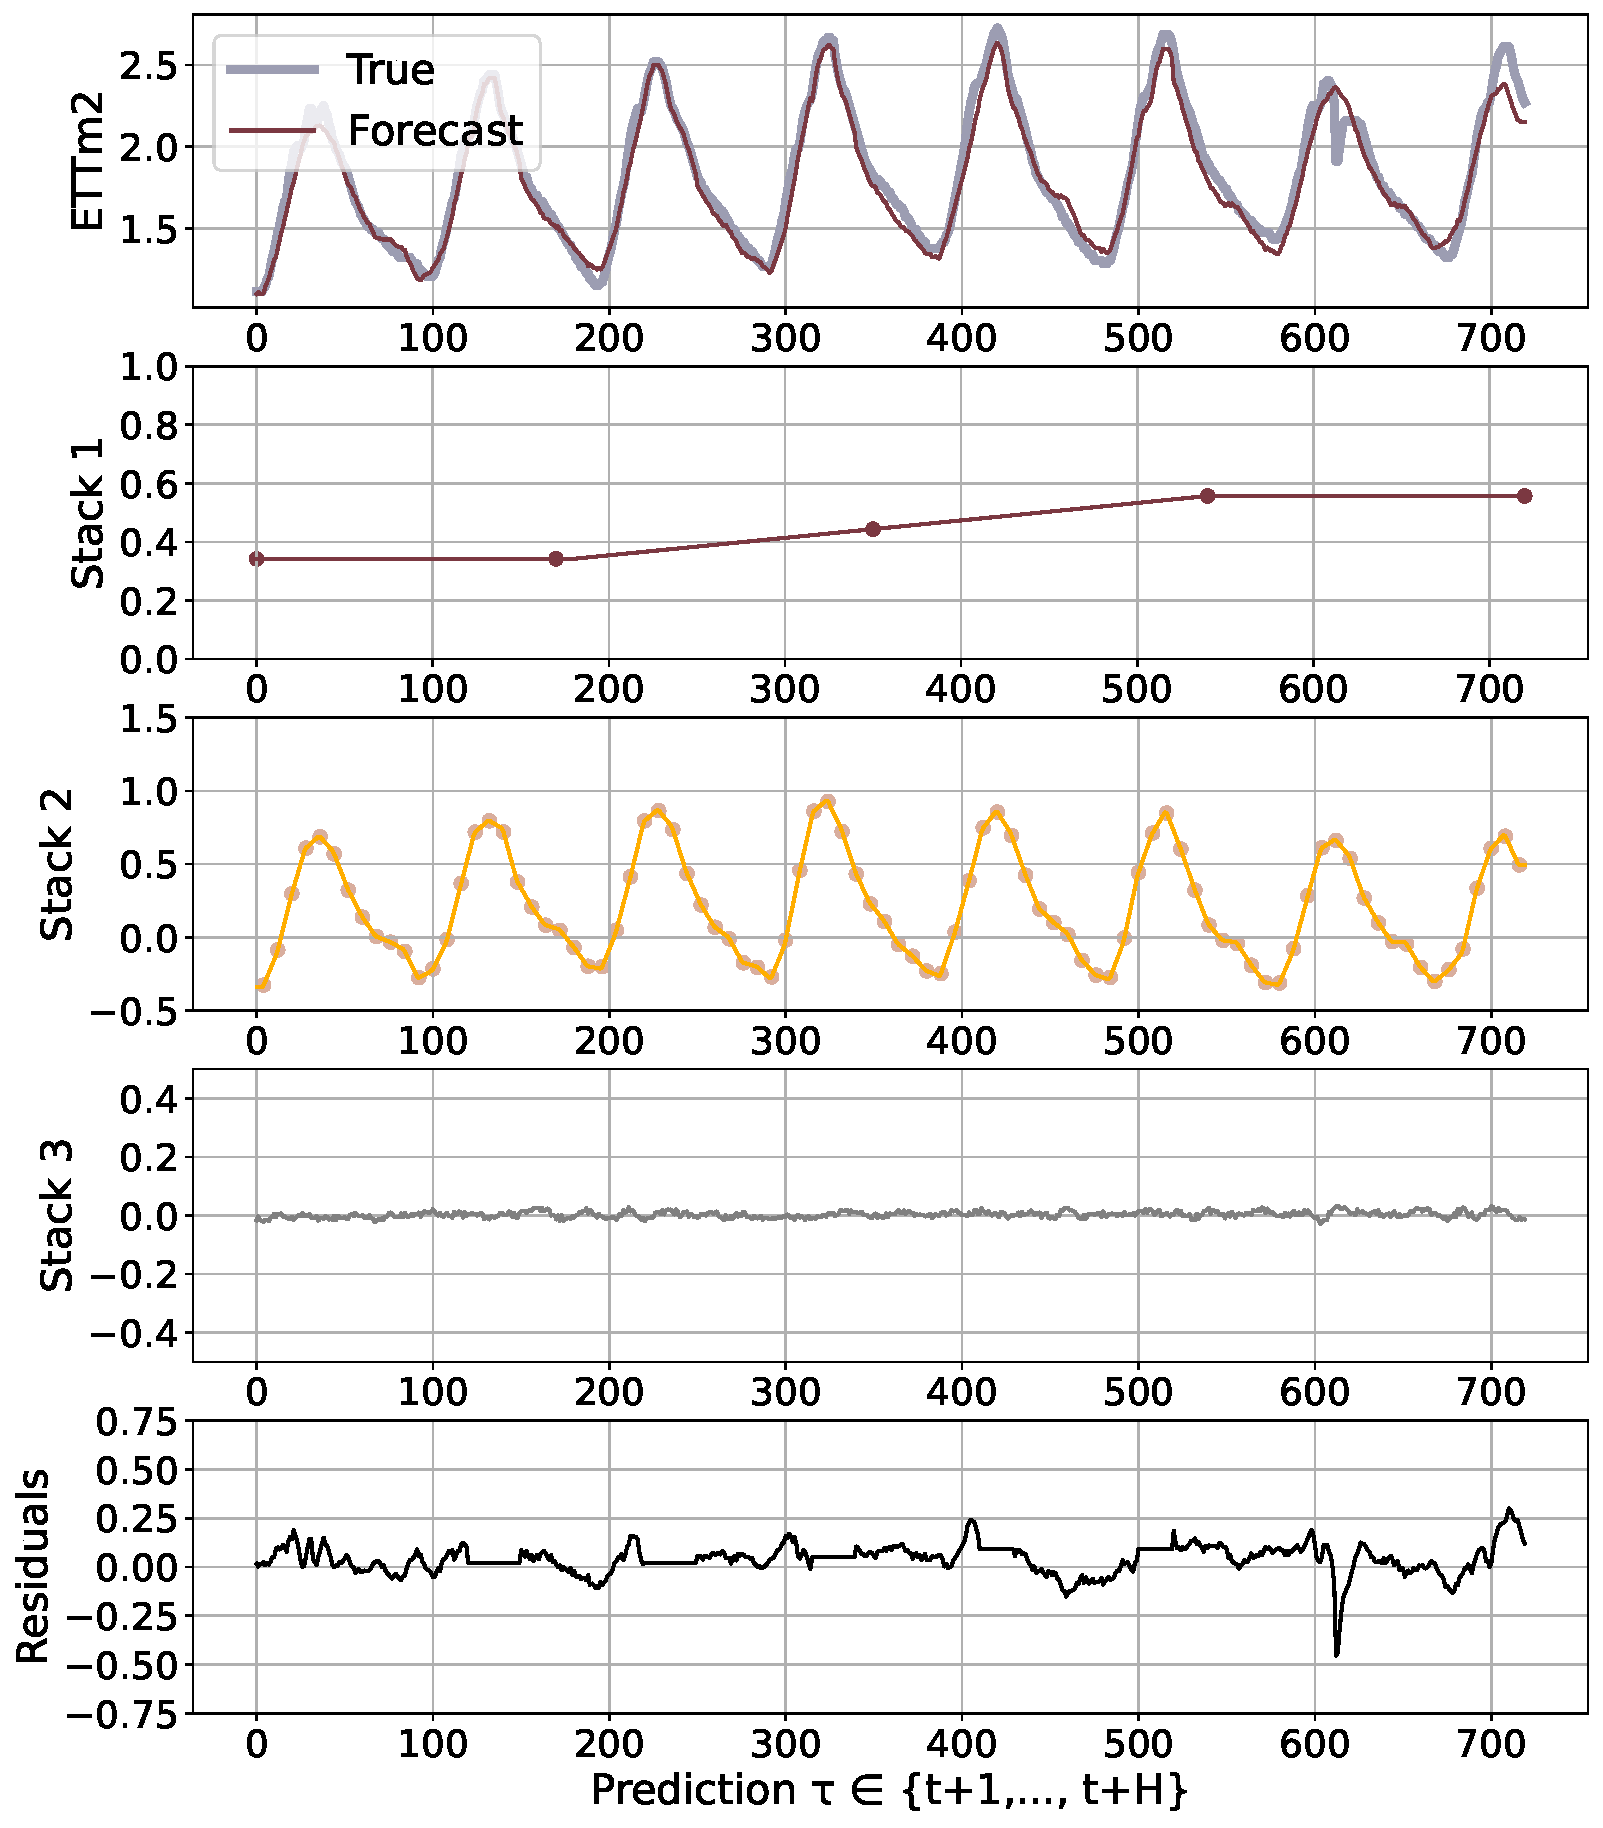
\includegraphics[width=0.3\linewidth]{images/plots-interpetable-decomposition.pdf}}
\subfigure[No h. interpolation, multi-rate sampling]{\label{fig:decomposition_g}
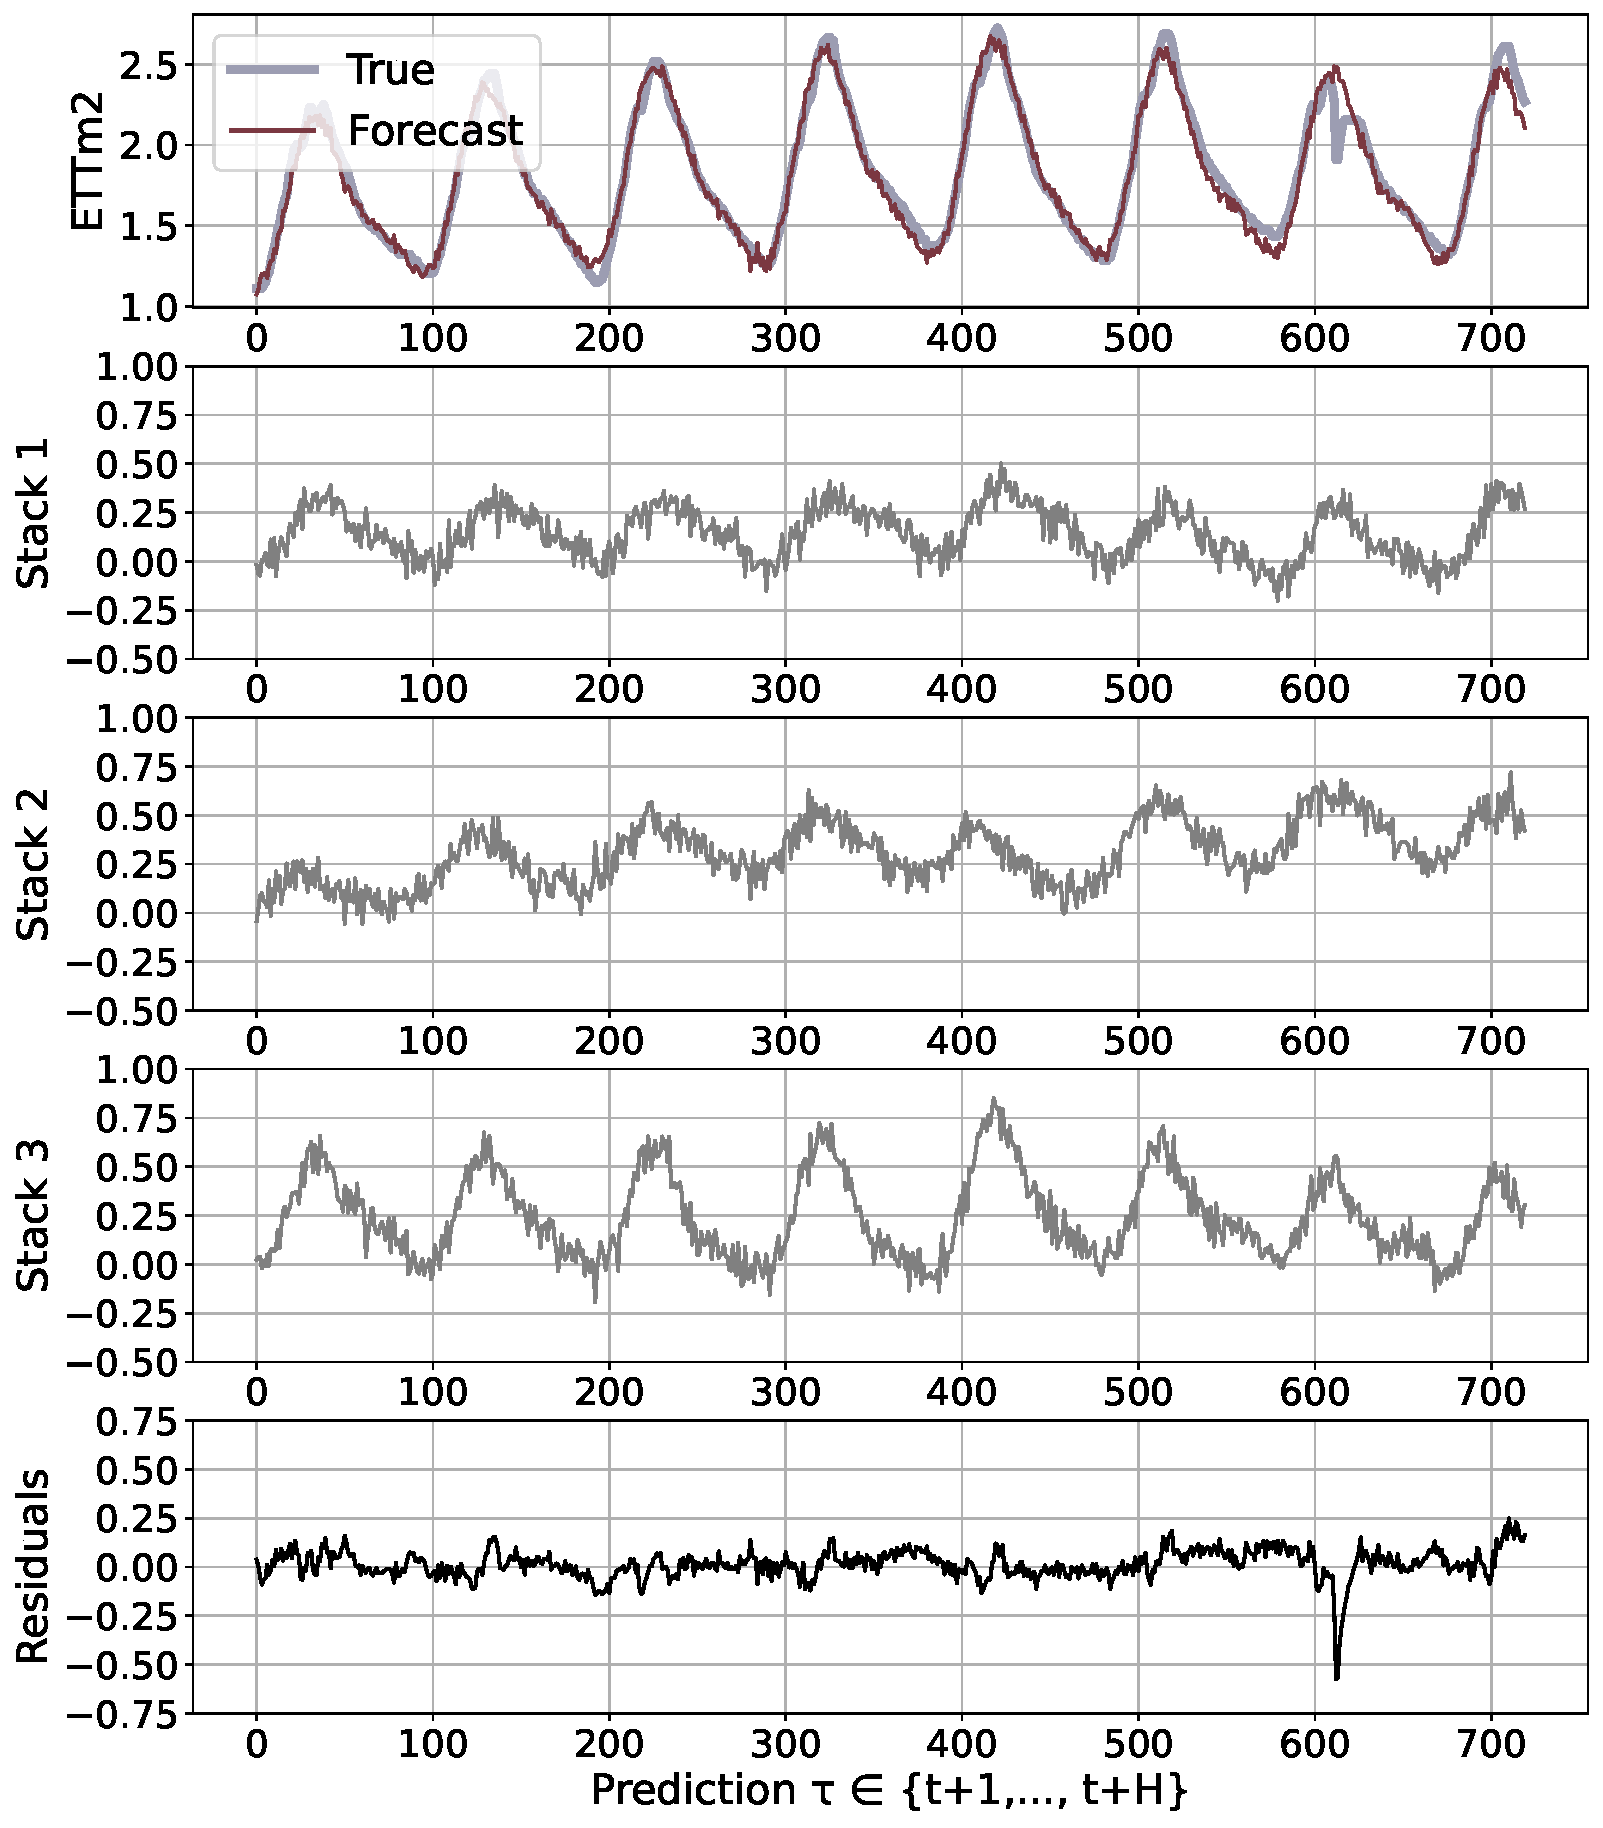
\includegraphics[width=0.3\linewidth]{images/plots-interpetable-decomposition-generic.pdf}}
\vspace{-0.25cm}
\caption{ETTm2 and 720 ahead forecasts using \ours\ (left panel), \ours\ with hierarchical linear interpolation and multi-rate sampling removed (right panel). The top row shows the original signal and the forecast. The second, third and fourth rows show the forecast components for each stack. The last row shows the residuals, $y-\hat{y}$. In (a), each block shows scale specialization, unlike (b), in which signals are not interpretable.} 
\label{fig:decomposition} %\textcolor{green}{FINAL}
\end{figure*}

\textbf{Computational Efficiency.} We measure the computational training time of \ours, \NBEATS\ and Transformer-based methods in the multivariate setting and show compare in Figure~\ref{fig:computational_cost_comparison}. The experiment monitors the whole training process for the \ETTm$_2$ dataset. For the Transformer-based models we used hyperparameters reported in \citep{wu2021autoformer}. Compared to the Transformer-based methods, \ours\ is \inferenceGains$\times$ faster than \Autoformer. In terms of memory, \ours\ has less than \memoryGains\% \ of the parameters of the second-best alternative, since it scales linearly with respect to the input's length. Compared to the original \NBEATS, our method is \inferenceGainsNBEATS$\times$ faster and requires only \memoryGainsNBEATS\% \ of the parameters. Finally, while \ours\ is an univariate model, it has \textit{global} (shared) parameters for all time-series in the dataset. Just like \cite{oreshkin2020nbeats}, our experiments (Appendix I) show that \ours\ maintains constant parameter/training computational complexity regarding dataset's size.

\subsection{Training and Hyperparameter Optimization}
\label{section:training_methodology}

We consider a minimal space of hyperparameters to explore configurations of the \ours\ architecture.
First, we consider the kernel pooling size for multi-rate sampling from Equation~(\ref{equation:nhits_mixed_datasampling}).
Second, the number of coefficients from Equation~(\ref{equation:nhits_projections}) that we selected between several alternatives, some matching common seasonalities of the datasets and others exponentially increasing. We tune the random seed to escape underperforming local minima. Details are reported in Table A3 in Appendix D.

During the \emph{hyperparameter optimization phase}, we measure MAE performance on the validation set and use a Bayesian optimization library (\HYPEROPT;\,\citealt{bergstra2011hyperopt}), with 20 iterations. We use the optimal configuration based on the validation loss to make prediction on the test set. We refer to the combination of hyperparameter optimization and test prediction as a \emph{run}. \ours\ is implemented in \PyTorch~\citep{pytorch2019library} and trained using \ADAM\ optimizer~\citep{kingma2014adam_method}, MAE loss, batch size 256 and initial learning rate of 1e-3, halved three times across the training procedure. All our experiments are conducted on a GeForce RTX 2080 GPU.

\subsection{Ablation Studies}
\label{appendix:ablation_main_contributions}

We believe that the advantages of the \ours\ architecture are rooted in its multi-rate hierarchical nature. Fig.~\ref{fig:decomposition} shows a qualitative comparison of \ours\ with and without hierarchical interpolation/multi-rate sampling components. We clearly see \ours\ developing the ability to produce interpretable forecast decomposition providing valuable information about trends and seasonality in separate channels, unlike the control model. Appendix G presents the decomposition for the different interpolation techniques. We support our qualitative conclusion with quantitative results. We define the following set of alternative models: \ours, our proposed model with both multi-rate sampling and hierarchical interpolation, \ours$_{2}$ only hierarchical interpolation, \ours$_{3}$ only multi-rate sampling, \ours$_{4}$ no multi-rate sampling or interpolation (corresponds to the original \NBEATSg~\citep{oreshkin2020nbeats}), finally \NBEATSi, the interpreatble version of the \NBEATS\ (\citep{oreshkin2020nbeats}). Tab.~\ref{table:ablation_nhits_contributions} clearly shows that the combination of both proposed components (hierarchical interpolation and multi-rate sampling) results in the best performance, emphasizing their complementary nature in long-horizon forecasting. We see that the original \NBEATS\ is consistently worse, especially the \NBEATSi. The advantages of the proposed techniques for long-horizon forecasting, multi-rate sampling and interpolation, are not limited to the \ours\ architecture. In Appendix H we demonstrate how adding them to a \DilRNN\ improve its performance.

\begin{table}[ht!] 
% \tiny
\scriptsize
    \begin{center}
    \caption{Empirical evaluation of long multi-horizon multivariate forecasts for \ours\ with/without enhancements. MAE and MSE for predictions averaged over eight runs, and five datasets, the best result is highlighted in bold, second best in blue (lower is better).}
    \label{table:ablation_nhits_contributions}
	\begin{tabular}{ll | ccccc} \toprule
    						&     & \ours                    & \ours$_{2}$             & \ours$_{3}$              & \ours$_{4}$ & \NBEATSi \\ \midrule
\parbox[t]{1mm}{\multirow{4}{*}{\rotatebox[origin=c]{90}{A. MSE}}}
							& 96  & \textcolor{blue}{0.195}  & 0.196                   & \textbf{0.192}           & 0.196       & 0.209    \\
							& 192 & \textbf{0.250}           & 0.261                   & \textcolor{blue}{0.251}  & 0.263       & 0.266    \\
							& 336 & \textbf{0.315}           & \textcolor{blue}{0.315} & 0.342                    & 0.346       & 0.408    \\
							& 720 & \textbf{0.484}           & \textcolor{blue}{0.498} & 0.518                    & 0.548       & 0.794    \\ \midrule
\parbox[t]{1mm}{\multirow{4}{*}{\rotatebox[origin=c]{90}{A. MAE}}}
							& 96  & \textcolor{blue}{0.239}  & 0.241                   & \textbf{0.237}           & 0.240       & 0.254   \\
							& 192 & \textbf{0.290}           & 0.299                   & \textcolor{blue}{0.291}  & 0.300       & 0.307   \\
							& 336 & \textbf{0.338}           & \textcolor{blue}{0.342} & 0.346                    & 0.352       & 0.405   \\
							& 720 & \textbf{0.439}           & \textcolor{blue}{0.450} & 0.454                    & 0.468       & 0.597   \\ \bottomrule
	\end{tabular}
	\end{center}
\end{table}

Additional \emph{ablation studies} are reported in Appendix G. The MaxPool multi-rate sampling wins over AveragePool. Linear interpolation wins over nearest neighbor and cubic. Finally and most importantly, we show that the order in which hierarchical interpolation is implemented matters significantly. The best configuration is to have the low-frequency/large-scale components  synthesized and removed from analysis first, followed by more fine-grained modeling of high-frequency/intermittent signals.